\begin{Ueberlieferung}% 
{\textit{L}}Reinschrift mit Verbesserungen: LH XXXVII 3 Bl. 79. 1 Bl. 4\textsuperscript{o} unregelmäßig beschnitten (ca 18 x 17 cm) mit zwei fehlenden Ecken. 1 S. auf Bl. 79~r\textsuperscript{o}. Bl. 79~v\textsuperscript{o} leer. Teil eines Wasserzeichens am Rand.\\%
Cc 2, Nr. 1213 C
\end{Ueberlieferung}
% \vspace*{8mm}
% \begin{Datierungsgruende}%
% ??
% \end{Datierungsgruende}
%
% \vspace*{2mm}
% \begin{ledgroup}
% \footnotesize 
% \pstart
% \noindent\footnotesize{\textbf{Datierungsgr\"{u}nde}: ?? Rest eines Wasserzeichens}
% \pend
% \end{ledgroup}
%
\vspace*{8mm}
% \begin{center}
% 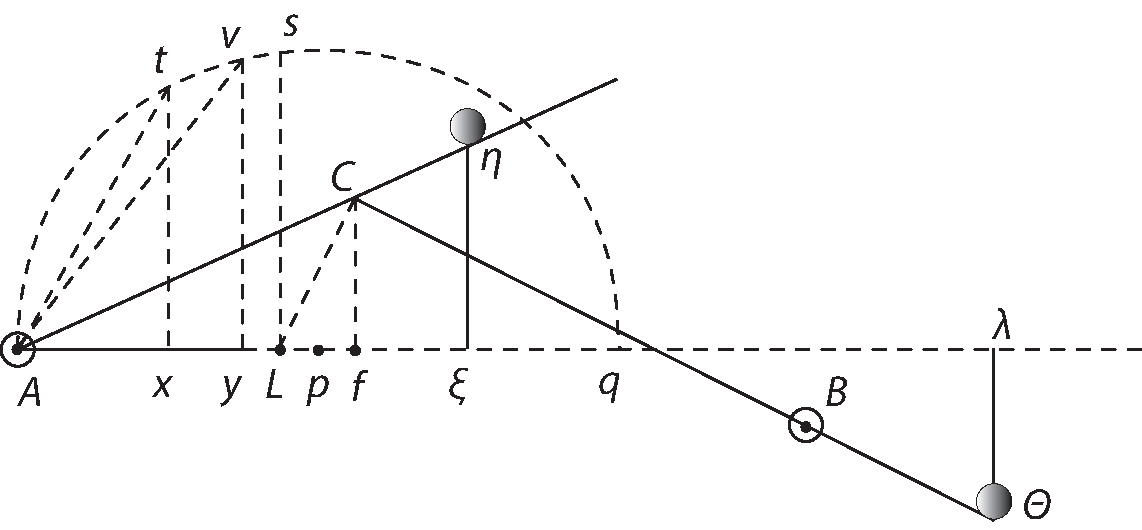
\includegraphics[width=0.8\textwidth]{images/LH037,03_079r-d1.pdf}\newline
% [\textit{Fig. 1}]
% \end{center}
% \vspace*{-5mm}
% \pstart\noindent
\count\Afootins=1200
\count\Bfootins=1200
\count\Cfootins=1200
\pstart\noindent
%\lbrack79~r\textsuperscript{o}\rbrack\ 
[79~r\textsuperscript{o}] 
Sunto duo vectes\protect\index{Sachverzeichnis}{vectis} conjugati $AC,$
\edtext{exterior seu qui impune produci potest}{\lemma{}\Bfootnote{exterior [...] potest, \textit{erg.} \textit{L}}}, et $BC$,
\edtext{interior}{\lemma{}\Bfootnote{interior: \textit{erg.} \textit{L}}}:
potentiae\protect\index{Sachverzeichnis}{potentia} sive
\edtext{%
pondera\protect\index{Sachverzeichnis}{pondus}
$\eta$ et $\theta$, $A\lambda$ recta transiens per centrum vectis\protect\index{Sachverzeichnis}{vectis} exterioris,
perpendicularis ad $\eta\xi$ lineam directionis potentiae\protect\index{Sachverzeichnis}{potentia} $\eta$ vel $\theta$
atque ideo horizontalis, si $\eta$ et $\theta$ pondera\protect\index{Sachverzeichnis}{pondus} esse intelligantur.
Potentiarum\protect\index{Sachverzeichnis}{potentia} altitudines sive distantiae ab $A\lambda$,
erunt $\eta\xi$ et $\theta\lambda$[,]%
}{\lemma{}\Bfootnote{pondera \textbar\ $\eta$ et $\theta$, \textit{erg.} \textbar\
\textit{(1)} altitudines ponderum $\eta\xi$ et $\theta\lambda$
\textit{(2)} $A\lambda$ recta [...] intelligantur.
\textit{(a)} Distantiae
\textit{(b)} Potentiarum [...] erunt $\eta\xi$ et $\theta\lambda$\ \textit{L}}}
punctum contactus $C,$ ejus altitudo $cf$
\edtext{et $CL$}{\lemma{}\Bfootnote{et $CL$ \textit{erg.} \textit{L}}} 
perpendicularis ad $BC,$ quae occurrat ipsi $A\lambda$ in $L.$ Esto porro $p$ punctum medium rectae $Lf,$ ac centro $p$ radio $pA$ 
\edtext{describatur circuli}{\lemma{describatur}\Bfootnote{\textit{(1)}\ circulus \textit{(2)}\ circuli \textit{L}}} 
semicircumferentia $ASq$ cui in puncto $S$ occurrat erecta ex $L$ normalis $LS.$ Transferatur $AC$ in $AV,$ et $LS$ in $AT,$ ut sint circuli descripti chordae. Demissis
\edtext{in diametrum}{\lemma{}\Bfootnote{in diametrum \textit{erg.} \textit{L}}} 
perpendicularibus $Tx,$ et $Vy,$ designabuntur \setline{11}rectae $Ax,$ et $Ay.$
\pend
\vspace{2em}
\pstart
\centering
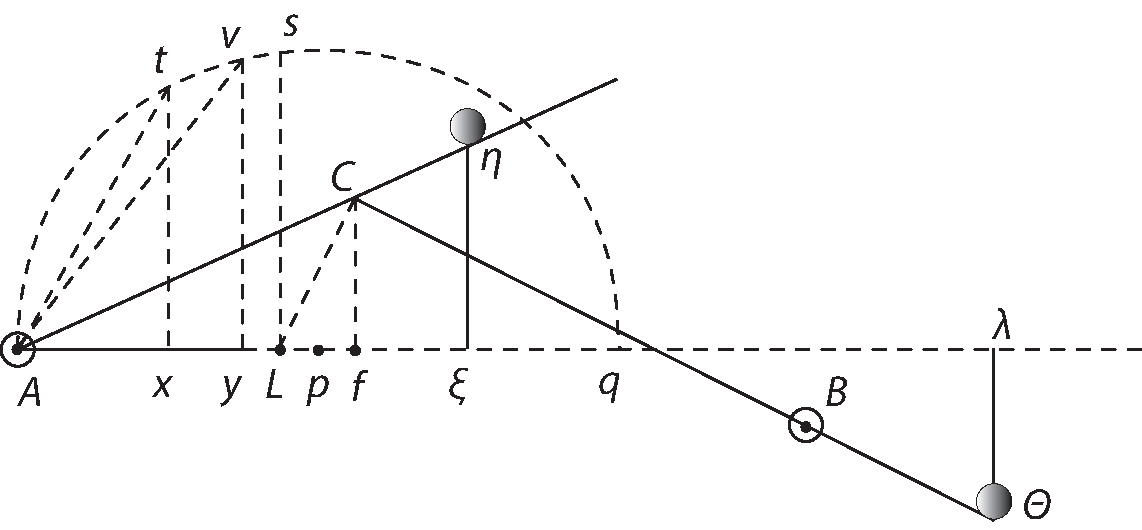
\includegraphics[width=0.78\textwidth]{images/LH037,03_079r-d1.pdf}\\
\centering
[\textit{Fig. 1}]
\pend
\newpage
\pstart
His ita praeparatis \edtext{ajo Rationem Virium quas exercent in se invicem potentiae\protect\index{Sachverzeichnis}{potentia} $\eta$ et $\theta$ esse compositam ex rationibus potentiarum\protect\index{Sachverzeichnis}{potentia} et altitudinum,%
}{\lemma{ajo}\Bfootnote{%
\textit{(1)} Vim quam exercet 
\textit{(2)} Rationem [...] invicem
\textit{(a)} pondera\protect\index{Sachverzeichnis}{pondus} $\eta$ et $\theta$ esse compositam ex 
\textit{(aa)} ratione inv
\textit{(bb)} rationibus,
\textbar\ directa \textit{erg.} \textbar\
ponderum,\protect\index{Sachverzeichnis}{pondus} et reciproca altitudinum,
\textit{(b)} potentiae\protect\index{Sachverzeichnis}{potentia} [...] altitudinum, \textit{L}}}
cum ratione rectarum $Ax$ et $Ay$. sive positis ponderibus\protect\index{Sachverzeichnis}{pondus} $\eta=a,$ et $\theta=\alpha,$ altitudinibus $\eta\xi=b,$ et $\theta\lambda=\beta,$ ac denique $Ay=d,$ et $Ax=\delta$ ac viribus, ponderis\protect\index{Sachverzeichnis}{pondus} quidem $a=x,$ ponderis\protect\index{Sachverzeichnis}{pondus}
\edtext{vero}{\lemma{}\Bfootnote{vero \textit{erg.} \textit{L}}}
$\alpha=\xi,$ fiet \rule[-4mm]{0mm}{10mm}$\displaystyle\frac{x}{\xi}=\frac{ab\delta}{\alpha\beta d}.$
\pend
\pstart
Et hoc quidem theorema\protect\index{Sachverzeichnis}{theorema} ad omnes casus definiendos, omniaque in hoc argumento problemata\protect\index{Sachverzeichnis}{problema} solvenda, ni fallor, sufficit.
\pend
\count\Afootins=1500
\count\Bfootins=1500
\count\Cfootins=1500